\section{积分}

\begin{problem}{函数在区间上的可积性判定}{Riemann-Integrability-Determination}
    指出下面的函数中哪些在区间 $[0, 1]$ 上可积？并说明理由．
    \begin{enumerate}
        \item $f(x) = \begin{dcases} \frac{\sin x}{x}, & x \neq 0, \\ 1, & x = 0; \end{dcases}$
        \item $f(x) = \begin{dcases} \frac{1}{x} \sin \frac{1}{x}, & x \neq 0, \\ 1, & x = 0; \end{dcases}$
        \item $f(x) = \begin{dcases} \frac{1}{\left[\frac{1}{x}\right]}, & 0 < x \leqslant 1, \\ 0, & x = 0. \end{dcases}$
    \end{enumerate}
\end{problem}

\begin{solution}
    \ansitem{1} 在 $[0, 1]$ 上可积．

    因为
    \begin{equation}
        \lim_{x\to 0^+} f(x) = \lim_{x\to 0^+} \frac{\sin x}{x} = 1 = f(0),
    \end{equation}
    所以函数 $f(x)$ 在闭区间 $[0, 1]$ 上连续．由闭区间上连续函数必可积的定理，函数 $f(x)$ 在 $[0, 1]$ 上 Riemann 可积．
    \begin{equation}
        \boxed{(1) \text{ 在 } [0, 1] \text{ 上可积．}}
    \end{equation}

    \ansitem{2} 在 $[0, 1]$ 上不可积．

    选取点列 $x_k = \frac{1}{2k\uppi + \frac{\uppi}{2}} \in (0, 1]$（$k \in \symbb{N}^+$），此时函数值为
    \begin{equation}
        f(x_k) = \left( 2k\uppi + \frac{\uppi}{2} \right) \sin\left( 2k\uppi + \frac{\uppi}{2} \right) = 2k\uppi + \frac{\uppi}{2} \to +\infty \quad (k \to \infty).
    \end{equation}
    函数 $f(x)$ 在区间 $[0, 1]$ 上无界．因为 Riemann 可积函数的必要条件是在该区间上有界，故 $f(x)$ 在 $[0, 1]$ 上不可积．
    \begin{equation}
        \boxed{(2) \text{ 在 } [0, 1] \text{ 上不可积．}}
    \end{equation}

    \ansitem{3} 在 $[0, 1]$ 上可积．

    当 $x \in \left( \frac{1}{k+1}, \frac{1}{k} \right]$（$k \in \symbb{N}^+$）时，$\left[\frac{1}{x}\right] = k$，故 $f(x) = \frac{1}{k}$．

    显然对任意 $x \in [0, 1]$ 恒有 $0 \leqslant f(x) \leqslant 1$，且当 $x_1 < x_2$ 时必有 $f(x_1) \leqslant f(x_2)$，即函数 $f(x)$ 在 $[0, 1]$ 上单调递增且有界．

    由有界单调函数必可积定理，函数 $f(x)$ 在 $[0, 1]$ 上 Riemann 可积．
    \begin{equation}
        \boxed{(3) \text{ 在 } [0, 1] \text{ 上可积．}}
    \end{equation}
\end{solution}

\begin{problem}{狄利克雷函数的不可积性}{Dirichlet-Function-Non-Integrability}
    证明 Dirichlet 函数在任意区间 $[a, b]$ 上不可积．（因此有界的函数未必可积．）
\end{problem}

\begin{myproof}
    Dirichlet 函数的定义为
    \begin{equation}
        D(x) = \begin{dcases} 1, & x \in \symbb{Q}, \\ 0, & x \in \symbb{R} \setminus \symbb{Q}. \end{dcases}
    \end{equation}
    对区间 $[a, b]$（$a < b$）的任意一个分割 $T : a = x_0 < x_1 < \cdots < x_n = b$，在每个小区间 $[x_{i-1}, x_i]$（$i = 1, 2, \cdots, n$）上：

    由有理数与无理数在实数集上的稠密性，小区间 $[x_{i-1}, x_i]$ 内既包含有理数也包含无理数，故
    \begin{equation}
        M_i = \sup_{x\in [x_{i-1}, x_i]} D(x) = 1, \qquad m_i = \inf_{x\in [x_{i-1}, x_i]} D(x) = 0.
    \end{equation}
    计算上 Darboux 和与下 Darboux 和：
    \begin{equation}
        S(T) = \sum_{i=1}^n M_i \Delta x_i = \sum_{i=1}^n 1 \cdot \Delta x_i = b - a,
    \end{equation}
    \begin{equation}
        s(T) = \sum_{i=1}^n m_i \Delta x_i = \sum_{i=1}^n 0 \cdot \Delta x_i = 0.
    \end{equation}
    因此，上积分与下积分分别为
    \begin{equation}
        \overline{\int_a^b} D(x) \d x = \inf_T S(T) = b - a,
    \end{equation}
    \begin{equation}
        \underline{\int_a^b} D(x) \d x = \sup_T s(T) = 0.
    \end{equation}
    因为 $a < b \implies b - a \neq 0$，上积分与下积分不相等：
    \begin{equation}
        \overline{\int_a^b} D(x) \d x \neq \underline{\int_a^b} D(x) \d x.
    \end{equation}
    故 Dirichlet 函数在任意区间 $[a, b]$ 上均不可积．
\end{myproof}

\begin{problem}{绝对值可积与原函数可积的反例}{Counterexample-Absolute-Integrability}
    举例说明，一个函数的绝对值函数在 $[a, b]$ 上可积，不能保证这函数在 $[a, b]$ 上可积．
\end{problem}

\begin{solution}
    在区间 $[a, b] = [0, 1]$ 上构造修改的 Dirichlet 函数：
    \begin{equation}
        f(x) = \begin{dcases} 1, & x \in \symbb{Q} \cap [0, 1], \\ -1, & x \in [0, 1] \setminus \symbb{Q}. \end{dcases}
    \end{equation}
    对其绝对值函数，对一切 $x \in [0, 1]$ 恒有
    \begin{equation}
        |f(x)| \equiv 1.
    \end{equation}
    常数函数 $|f(x)| = 1$ 在 $[0, 1]$ 上显然连续，因而 Riemann 可积，且 $\int_0^1 |f(x)| \d x = 1$．

    然而对原函数 $f(x)$，在 $[0, 1]$ 的任意分割 $T$ 下，每个小区间的确界为 $M_i = 1, m_i = -1$．上、下积分分别为
    \begin{equation}
        \overline{\int_0^1} f(x) \d x = 1, \qquad \underline{\int_0^1} f(x) \d x = -1.
    \end{equation}
    因上积分不等于下积分，函数 $f(x)$ 在 $[0, 1]$ 上不可积．
    \begin{equation}
        \boxed{f(x) = \begin{dcases} 1, & x \in \symbb{Q} \cap [0, 1], \\ -1, & x \in [0, 1] \setminus \symbb{Q}. \end{dcases}}
    \end{equation}
\end{solution}

\begin{problem}{非负函数积分的保号性与反例}{Non-Negative-Integrals-Positivity-And-Counterexample}
    \begin{enumerate}
        \item 设可积函数 $f(x)$ 在 $[a, b]$ 上非负，且在一点 $c$ 处连续（这里 $a \leqslant c \leqslant b$）．若 $f(c) > 0$，则 $\int_a^b f(x) \d x > 0$．
        \item 证明：若 $f(x)$ 是区间 $[a, b]$ 上非负的连续函数，且不恒为零，则 $\int_a^b f(x) \d x > 0$．
        \item 举例说明，有这样的可积函数 $f(x)$，在区间 $[a, b]$ 上非负且不恒为零，但 $f$ 在该区间上的积分为 $0$．
    \end{enumerate}
\end{problem}

\begin{solution}
    \ansitem{1}

    因为 $f(x)$ 在点 $c \in [a, b]$ 处连续且 $f(c) > 0$，取 $\varepsilon = \frac{f(c)}{2} > 0$．由连续性的局部保号性，存在 $\delta > 0$，使得当 $x \in [a, b] \cap [c - \delta, c + \delta]$ 时，恒有
    \begin{equation}
        f(x) > f(c) - \varepsilon = \frac{f(c)}{2}.
    \end{equation}
    区间 $[a, b] \cap [c - \delta, c + \delta]$ 包含一个非退化闭子区间 $[\alpha, \beta]$（$\alpha < \beta$）．

    利用定积分对区间的可加性与非负性（$f(x) \geqslant 0$），有
    \begin{equation}
        \begin{aligned}
            \int_a^b f(x) \d x & = \int_a^\alpha f(x) \d x + \int_\alpha^\beta f(x) \d x + \int_\beta^b f(x) \d x \\
                               & \geqslant 0 + \int_\alpha^\beta \frac{f(c)}{2} \d x + 0                          \\
                               & = \frac{f(c)}{2}(\beta - \alpha) > 0.
        \end{aligned}
    \end{equation}

    \ansitem{2}

    因为 $f(x)$ 在 $[a, b]$ 上非负且不恒为零，故存在一点 $c \in [a, b]$ 使得 $f(c) > 0$．

    又由于 $f(x)$ 在 $[a, b]$ 上处处连续，故 $f(x)$ 在点 $c$ 处连续且 $f(x)$ 在 $[a, b]$ 上 Riemann 可积．

    由 (1) 的结论，即得
    \begin{equation}
        \int_a^b f(x) \d x > 0.
    \end{equation}

    \ansitem{3}

    在区间 $[0, 1]$ 上构造函数
    \begin{equation}
        f(x) = \begin{dcases} 1, & x = 0, \\ 0, & x \in (0, 1]. \end{dcases}
    \end{equation}
    函数 $f(x)$ 在 $[0, 1]$ 上非负且 $f(0) = 1 \neq 0$（不恒为零）．

    由于 $f(x)$ 仅有 $x = 0$ 一个间断点，因而在 $[0, 1]$ 上 Riemann 可积，且
    \begin{equation}
        \int_0^1 f(x) \d x = 0.
    \end{equation}
    \begin{equation}
        \boxed{f(x) = \begin{dcases} 1, & x = 0, \\ 0, & x \in (0, 1]. \end{dcases}}
    \end{equation}
\end{solution}

\begin{problem}{单调函数定积分的不等式}{Monotone-Function-Integral-Inequalities}
    若函数 $f(x)$ 在 $[a, b]$ 上单调递增，则
    \begin{equation}
        (b - a)f(a) \leqslant \int_a^b f(x) \d x \leqslant (b - a)f(b).
    \end{equation}
    若 $f(x)$ 在 $[a, b]$ 上单调递减，应该有什么样的不等式？
\end{problem}

\begin{solution}
    先推导单调递增的情形：若 $f(x)$ 在 $[a, b]$ 上单调递增，则对任意 $x \in [a, b]$，恒有
    \begin{equation}
        f(a) \leqslant f(x) \leqslant f(b).
    \end{equation}
    由定积分的保序性定理，在各边从 $a$ 到 $b$ 积分，得
    \begin{equation}
        \int_a^b f(a) \d x \leqslant \int_a^b f(x) \d x \leqslant \int_a^b f(b) \d x,
    \end{equation}
    即
    \begin{equation}
        (b - a)f(a) \leqslant \int_a^b f(x) \d x \leqslant (b - a)f(b).
    \end{equation}
    若 $f(x)$ 在 $[a, b]$ 上单调递减，则对任意 $x \in [a, b]$，恒有
    \begin{equation}
        f(b) \leqslant f(x) \leqslant f(a).
    \end{equation}
    同理在各边积分，即得相应的不等式：
    \begin{equation}
        (b - a)f(b) \leqslant \int_a^b f(x) \d x \leqslant (b - a)f(a).
    \end{equation}
    \begin{equation}
        \boxed{(b - a)f(b) \leqslant \int_a^b f(x) \d x \leqslant (b - a)f(a).}
    \end{equation}
\end{solution}

\begin{problem}{定积分的估值不等式}{Definite-Integral-Estimation-Inequalities}
    证明下列不等式：
    \begin{enumerate}
        \item $\int_0^{2\uppi} |a\sin x + b\cos x| \d x \leqslant 2\uppi\sqrt{a^2 + b^2}$（$a, b$ 为常数）；
        \item $\int_0^1 x^m (1 - x)^n \d x \leqslant \frac{m^m n^n}{(m + n)^{m+n}}$（$m > 0, n > 0$，均为常数）．
    \end{enumerate}
\end{problem}

\begin{myproof}
    \ansitem{1}

    由 Cauchy-Schwarz 不等式（或辅助角公式），对任意实数 $x$，有
    \begin{equation}
        |a\sin x + b\cos x| \leqslant \sqrt{a^2 + b^2} \sqrt{\sin^2 x + \cos^2 x} = \sqrt{a^2 + b^2}.
    \end{equation}
    在区间 $[0, 2\uppi]$ 上对两端取定积分，由定积分保序性得
    \begin{equation}
        \int_0^{2\uppi} |a\sin x + b\cos x| \d x \leqslant \int_0^{2\uppi} \sqrt{a^2 + b^2} \d x = 2\uppi\sqrt{a^2 + b^2}.
    \end{equation}

    \ansitem{2}

    考虑函数 $g(x) = x^m (1 - x)^n$ 在闭区间 $[0, 1]$ 上的最值．求导得
    \begin{equation}
        \begin{aligned}
            g'(x) & = m x^{m-1}(1 - x)^n - n x^m(1 - x)^{n-1}          \\
                  & = x^{m-1}(1 - x)^{n-1}\bigl[ m(1 - x) - n x \bigr] \\
                  & = x^{m-1}(1 - x)^{n-1}\bigl[ m - (m + n)x \bigr].
        \end{aligned}
    \end{equation}
    令 $g'(x) = 0$，在区间 $(0, 1)$ 内解得唯一驻点 $x_0 = \frac{m}{m + n}$．

    当 $x \in (0, x_0)$ 时 $g'(x) > 0$；当 $x \in (x_0, 1)$ 时 $g'(x) < 0$．故函数 $g(x)$ 在 $x = x_0$ 处取得在 $[0, 1]$ 上的全局最大值：
    \begin{equation}
        \max_{x\in [0, 1]} g(x) = g\left( \frac{m}{m + n} \right) = \left( \frac{m}{m + n} \right)^m \left( \frac{n}{m + n} \right)^n = \frac{m^m n^n}{(m + n)^{m+n}}.
    \end{equation}
    因此对一切 $x \in [0, 1]$，恒有
    \begin{equation}
        x^m (1 - x)^n \leqslant \frac{m^m n^n}{(m + n)^{m+n}}.
    \end{equation}
    在区间 $[0, 1]$ 上对两端取定积分，得
    \begin{equation}
        \int_0^1 x^m (1 - x)^n \d x \leqslant \int_0^1 \frac{m^m n^n}{(m + n)^{m+n}} \d x = \frac{m^m n^n}{(m + n)^{m+n}} (1 - 0) = \frac{m^m n^n}{(m + n)^{m+n}}.
    \end{equation}
\end{myproof}

\begin{problem}{积分中值定理的中值范围与连续性必要性}{Integral-Mean-Value-Theorem-Interior-Point-And-Continuity}
    \begin{enumerate}
        \item 证明：积分中值定理中的中值 $\xi$，可取在区间 $[a, b]$ 内部．
              （提示：由这定理的证明可见，只要指出当 $f$ 的最大值 $M$ 或最小值 $m$ 在区间端点取得，且等于 $\frac{1}{b-a}\int_a^b f(x)\d x$ 时，结论成立．）
        \item 举例说明，积分中值定理中连续性的条件是必要的．
    \end{enumerate}

    \textbf{附定理 5.11（积分中值定理）}：设函数 $f(x)$ 在闭区间 $[a, b]$ 上连续，则存在 $\xi \in [a, b]$，使得
    \begin{equation}
        \int_a^b f(x)\d x = f(\xi)(b-a).
    \end{equation}
\end{problem}

\begin{solution}
    \ansitem{1}

    若 $f(x)$ 在 $[a, b]$ 上为常数函数，即 $f(x) \equiv C$，则对任意 $\xi \in (a, b)$，恒有
    \begin{equation}
        f(\xi)(b - a) = C(b - a) = \int_a^b f(x)\d x,
    \end{equation}
    结论显然成立．

    若 $f(x)$ 不恒为常数，由闭区间上连续函数的最大值最小值定理，存在 $m, M$ 使得
    \begin{equation}
        m = \min_{x\in [a, b]} f(x), \qquad M = \max_{x\in [a, b]} f(x),
    \end{equation}
    且必有 $m < M$．

    由于连续函数 $f(x) - m \geqslant 0$ 且不恒为零，由非负连续函数的积分性质，有
    \begin{equation}
        \int_a^b \bigl( f(x) - m \bigr)\d x > 0 \implies \frac{1}{b-a}\int_a^b f(x)\d x > m.
    \end{equation}
    同理，由于 $M - f(x) \geqslant 0$ 且不恒为零，有
    \begin{equation}
        \int_a^b \bigl( M - f(x) \bigr)\d x > 0 \implies \frac{1}{b-a}\int_a^b f(x)\d x < M.
    \end{equation}
    因此实数 $\mu = \frac{1}{b-a}\int_a^b f(x)\d x$ 严格介于最小值与最大值之间：
    \begin{equation}
        m < \mu < M.
    \end{equation}
    设 $f(x)$ 分别在 $x_1, x_2 \in [a, b]$ 处取得最小值与最大值，即 $f(x_1) = m$，$f(x_2) = M$．

    由连续函数的介值定理，在以 $x_1$ 与 $x_2$ 为端点的开子区间内必存在一点 $\xi \in (a, b)$，使得
    \begin{equation}
        f(\xi) = \mu = \frac{1}{b-a}\int_a^b f(x)\d x \implies \int_a^b f(x)\d x = f(\xi)(b-a).
    \end{equation}

    \ansitem{2}

    考虑在闭区间 $[0, 1]$ 上的分段函数
    \begin{equation}
        f(x) = \begin{dcases} 1, & x \in \left[0, \frac{1}{2}\right], \\ 2, & x \in \left(\frac{1}{2}, 1\right]. \end{dcases}
    \end{equation}
    函数 $f(x)$ 在 $[0, 1]$ 上有界且仅有 $x = \frac{1}{2}$ 一个间断点，因而 Riemann 可积．计算其定积分：
    \begin{equation}
        \int_0^1 f(x)\d x = \int_0^{1/2} 1\d x + \int_{1/2}^1 2\d x = 1 \cdot \frac{1}{2} + 2 \cdot \frac{1}{2} = \frac{3}{2}.
    \end{equation}
    然而函数 $f(x)$ 的值域为 $\{1, 2\}$，对任意 $\xi \in [0, 1]$，恒有 $f(\xi) \neq \frac{3}{2}$，即不存在任何 $\xi \in [0, 1]$ 满足
    \begin{equation}
        f(\xi)(1 - 0) = \int_0^1 f(x)\d x = \frac{3}{2}.
    \end{equation}
    这说明积分中值定理中函数连续性的条件是必不可少的．
    \begin{equation}
        \boxed{f(x) = \begin{dcases} 1, & x \in \left[0, \frac{1}{2}\right], \\ 2, & x \in \left(\frac{1}{2}, 1\right]. \end{dcases}}
    \end{equation}
\end{solution}

\begin{problem}{定积分为零的连续函数的零点存在性}{Continuous-Function-With-Zero-Integral-Zero-Point}
    设 $f$ 是区间 $[a, b]$ 上的连续函数．若 $\int_a^b f(x)\d x = 0$，则 $f$ 在 $(a, b)$ 中至少有一个零点．（因此，由函数的积分这一整体信息，能够推断函数值的某些性质．）
\end{problem}

\begin{myproof}
    若 $f(x) \equiv 0$，则开区间 $(a, b)$ 内的每一点均为零点，结论显然成立．

    若 $f(x) \not\equiv 0$：采用反证法．假设 $f(x)$ 在 $(a, b)$ 内没有零点．

    由闭区间上连续函数的介值定理，函数 $f(x)$ 在开区间 $(a, b)$ 内恒保持同号．

    不妨设对一切 $x \in (a, b)$ 恒有 $f(x) > 0$（恒负的情形完全对称）．

    由极限的保号性，在端点处有
    \begin{equation}
        f(a) = \lim_{x\to a^+} f(x) \geqslant 0, \qquad f(b) = \lim_{x\to b^-} f(x) \geqslant 0.
    \end{equation}
    因此 $f(x)$ 是闭区间 $[a, b]$ 上的非负连续函数，且不恒为零．

    由非负连续函数的积分性质，必有
    \begin{equation}
        \int_a^b f(x)\d x > 0,
    \end{equation}
    这与已知条件 $\int_a^b f(x)\d x = 0$ 产生矛盾．

    故假设不成立，函数 $f(x)$ 在开区间 $(a, b)$ 内至少有一个零点．
\end{myproof}

\begin{problem}{加权积分中值定理及其条件分析}{Weighted-Mean-Value-Theorem-For-Integrals}
    \begin{enumerate}
        \item 设函数 $f(x)$ 在 $[a, b]$ 上连续，而 $g(x)$ 在 $[a, b]$ 上可积且是非负（或非正）的．证明：存在 $\xi \in [a, b]$，使得
              \begin{equation}
                  \int_a^b f(x)g(x)\d x = f(\xi)\int_a^b g(x)\d x.
              \end{equation}
        \item 举例说明，(1) 中对于函数 $g$ 的假设是必不可少的．
    \end{enumerate}
    注 (1) 中的结果也称为积分中值定理的加权推广．这种加权的积分中值定理，也提供了估计积分的一个手段：当 $\int_a^b \varphi(x)\d x$ 不易计算时，可试作将 $\varphi(x)$ 写成 $f(x)g(x)$，其中 $f(x)$ 和 $g(x)$ 满足上面 (1) 中的条件，且使得 $\int_a^b g(x)\d x$ 易于计算．由此导出
    \begin{equation}
        m \int_a^b g(x)\d x \leqslant \int_a^b \varphi(x)\d x \leqslant M \int_a^b g(x)\d x,
    \end{equation}
    这里 $M, m$ 分别是 $f(x)$ 在 $[a, b]$ 上的最大值及最小值．易于看到，$\int_a^b \varphi(x)\d x$ 这一上、下界估计，优于直接用定理 5.11 所得的结果．

    \textbf{附定理 5.11（积分中值定理）}：设函数 $f(x)$ 在闭区间 $[a, b]$ 上连续，则存在 $\xi \in [a, b]$，使得
    \begin{equation}
        \int_a^b f(x)\d x = f(\xi)(b-a).
    \end{equation}
\end{problem}

\begin{solution}
    \ansitem{1}

    不妨设 $g(x) \geqslant 0$（非正的情形完全对称）．

    因为 $f(x)$ 在闭区间 $[a, b]$ 上连续，由最大值最小值定理，存在 $m, M$ 使得
    \begin{equation}
        m = \min_{x\in [a, b]} f(x), \qquad M = \max_{x\in [a, b]} f(x).
    \end{equation}
    即对任意 $x \in [a, b]$，恒有 $m \leqslant f(x) \leqslant M$．

    由于 $g(x) \geqslant 0$，同乘 $g(x)$ 得
    \begin{equation}
        m g(x) \leqslant f(x)g(x) \leqslant M g(x).
    \end{equation}
    由定积分的保序性，在区间 $[a, b]$ 上积分得
    \begin{equation}
        m \int_a^b g(x)\d x \leqslant \int_a^b f(x)g(x)\d x \leqslant M \int_a^b g(x)\d x.
    \end{equation}
    分情况讨论：
    \begin{enumerate}
        \item 若 $\int_a^b g(x)\d x = 0$，由上式可得 $\int_a^b f(x)g(x)\d x = 0$，等式对任意 $\xi \in [a, b]$ 均显然成立；
        \item 若 $\int_a^b g(x)\d x > 0$，两端同除以 $\int_a^b g(x)\d x$，得
              \begin{equation}
                  m \leqslant \frac{\int_a^b f(x)g(x)\d x}{\int_a^b g(x)\d x} \leqslant M.
              \end{equation}
              由连续函数的介值定理，存在 $\xi \in [a, b]$，使得
              \begin{equation}
                  f(\xi) = \frac{\int_a^b f(x)g(x)\d x}{\int_a^b g(x)\d x} \implies \int_a^b f(x)g(x)\d x = f(\xi)\int_a^b g(x)\d x.
              \end{equation}
    \end{enumerate}

    \ansitem{2}

    在闭区间 $[-1, 1]$ 上取连续函数 $f(x) = x$，并取变号函数 $g(x) = x$（在 $[-1, 1]$ 上可积但非定号）．

    计算等式左端：
    \begin{equation}
        \int_{-1}^1 f(x)g(x)\d x = \int_{-1}^1 x^2 \d x = \frac{2}{3}.
    \end{equation}
    计算等式右端：
    \begin{equation}
        \int_{-1}^1 g(x)\d x = \int_{-1}^1 x\d x = 0.
    \end{equation}
    对任意 $\xi \in [-1, 1]$，右端恒为
    \begin{equation}
        f(\xi)\int_{-1}^1 g(x)\d x = f(\xi) \cdot 0 = 0.
    \end{equation}
    因为 $\frac{2}{3} \neq 0$，不存在任何 $\xi \in [-1, 1]$ 满足等式．

    故 $g(x)$ 在区间上保持定号的条件是必不可少的．
    \begin{equation}
        \boxed{f(x) = x, \quad g(x) = x, \quad x \in [-1, 1].}
    \end{equation}
\end{solution}

\begin{problem}{变上限积分可导与被积函数连续性的关系}{Differentiability-Of-Variable-Upper-Limit-Integral}
    举例说明：在定理 5.13 中，函数 $f(x)$ 在 $x = c$ 处连续，不是 $F(x) = \int_a^x f(t)\d t$ 在 $x = c$ 处可导的必要条件．

    \textbf{附定理 5.13 内容}：设函数 $f(x)$ 在 $[a, b]$ 上可积，$x_0 \in [a, b]$．
    \begin{enumerate}
        \item 若 $f(x)$ 在 $x = x_0$ 处连续，则 $f(x)$ 的变上限积分 $\varphi$ 在 $x = x_0$ 处可微，且 $\varphi'(x_0) = f(x_0)$．
        \item 若 $f(x)$ 在区间 $[a, b]$ 上连续，则 $f(x)$ 的变上限积分在 $[a, b]$ 上可微，并且
              \begin{equation}
                  \varphi'(x) = f(x), \quad a \leqslant x \leqslant b, \quad \text{或} \quad \d\varphi(x) = \d\int_a^x f(t)\d t = f(x)\d x,
              \end{equation}
              即 $\varphi(x)$ 是 $f(x)$ 的一个原函数．所以我们也有这样的结论：连续函数一定有原函数．
    \end{enumerate}
\end{problem}

\begin{solution}
    在闭区间 $[0, 1]$ 上构造函数
    \begin{equation}
        f(t) = \begin{dcases} 1, & t \neq \frac{1}{2}, \\ 0, & t = \frac{1}{2}, \end{dcases}
    \end{equation}
    并取考察点 $c = \frac{1}{2}$．

    函数 $f(t)$ 在 $t = \frac{1}{2}$ 处不连续（$t = \frac{1}{2}$ 为第一类可去间断点，$\lim_{t\to 1/2} f(t) = 1 \neq f\left(\frac{1}{2}\right) = 0$）．

    由于改变有限个点的值不改变定积分的值，其变上限积分函数为
    \begin{equation}
        F(x) = \int_0^x f(t)\d t = \int_0^x 1\d t = x, \quad x \in [0, 1].
    \end{equation}
    函数 $F(x) = x$ 在点 $c = \frac{1}{2}$ 处显然可导，且导数值为
    \begin{equation}
        F'\left(\frac{1}{2}\right) = 1.
    \end{equation}
    这表明即使被积函数 $f(x)$ 在点 $c$ 处不连续，变上限积分 $F(x)$ 在点 $c$ 处仍然可以可导．故被积函数在 $x = c$ 处连续不是变上限积分可导的必要条件．
    \begin{equation}
        \boxed{f(t) = \begin{dcases} 1, & t \neq \frac{1}{2}, \\ 0, & t = \frac{1}{2}, \end{dcases} \quad c = \frac{1}{2}.}
    \end{equation}
\end{solution}

\begin{problem}{变限积分函数的求导}{Derivative-Of-Variable-Limit-Integrals}
    求下列函数的导数：
    \begin{enumerate}
        \item $f(x) = \int_0^{x^2} \sin t^2 \d t$；
        \item $f(x) = \int_x^1 \frac{1}{1 + t^2 + \cos^2 t} \d t$；
        \item $f(x) = \int_x^{x^2} \e^{-t^2} \d t$；
        \item $f(x) = \sin\left( \int_0^x \sin\left( \int_0^y \sin t^2 \d t \right) \d y \right)$．
    \end{enumerate}
\end{problem}

\begin{solution}
    \ansitem{1}

    由变上限积分求导法则与复合函数求导法则：
    \begin{equation}
        f'(x) = \sin\bigl((x^2)^2\bigr) \cdot (x^2)' = 2x \sin(x^4).
    \end{equation}
    \begin{equation}
        \boxed{f'(x) = 2x \sin(x^4).}
    \end{equation}

    \ansitem{2}

    交换积分上下限：
    \begin{equation}
        f(x) = -\int_1^x \frac{1}{1 + t^2 + \cos^2 t} \d t.
    \end{equation}
    求导得
    \begin{equation}
        f'(x) = -\frac{1}{1 + x^2 + \cos^2 x}.
    \end{equation}
    \begin{equation}
        \boxed{f'(x) = -\frac{1}{1 + x^2 + \cos^2 x}.}
    \end{equation}

    \ansitem{3}

    拆分为两个变限积分：
    \begin{equation}
        f(x) = \int_0^{x^2} \e^{-t^2} \d t - \int_0^x \e^{-t^2} \d t.
    \end{equation}
    求导得
    \begin{equation}
        f'(x) = \e^{-(x^2)^2} \cdot (x^2)' - \e^{-x^2} = 2x \e^{-x^4} - \e^{-x^2}.
    \end{equation}
    \begin{equation}
        \boxed{f'(x) = 2x \e^{-x^4} - \e^{-x^2}.}
    \end{equation}

    \ansitem{4}

    由复合函数求导法则：
    \begin{equation}
        \begin{aligned}
            f'(x) & = \cos\left( \int_0^x \sin\left( \int_0^y \sin t^2 \d t \right) \d y \right) \cdot \frac{\d}{\d x}\left( \int_0^x \sin\left( \int_0^y \sin t^2 \d t \right) \d y \right) \\
                  & = \cos\left( \int_0^x \sin\left( \int_0^y \sin t^2 \d t \right) \d y \right) \sin\left( \int_0^x \sin t^2 \d t \right).
        \end{aligned}
    \end{equation}
    \begin{equation}
        \boxed{f'(x) = \cos\left( \int_0^x \sin\left( \int_0^y \sin t^2 \d t \right) \d y \right) \sin\left( \int_0^x \sin t^2 \d t \right).}
    \end{equation}
\end{solution}

\begin{problem}{反函数的导数与变限积分}{Derivative-Of-Inverse-Function}
    对下面的函数，求 $(f^{-1})'(0)$，这里 $f^{-1}(x)$ 表示函数 $f(x)$ 的反函数：
    \begin{enumerate}
        \item $f(x) = \int_0^x [1 + \sin(\sin t)] \d t$；
        \item $f(x) = \int_1^x \e^{-t^2} \d t$．
    \end{enumerate}
\end{problem}

\begin{solution}
    \ansitem{1}

    由定义知 $f(0) = 0$，故 $f^{-1}(0) = 0$．

    对 $f(x)$ 求导得
    \begin{equation}
        f'(x) = 1 + \sin(\sin x) \implies f'(0) = 1 + \sin(0) = 1 \neq 0.
    \end{equation}
    由反函数求导公式，得
    \begin{equation}
        (f^{-1})'(0) = \frac{1}{f'(f^{-1}(0))} = \frac{1}{f'(0)} = \frac{1}{1} = 1.
    \end{equation}
    \begin{equation}
        \boxed{(f^{-1})'(0) = 1.}
    \end{equation}

    \ansitem{2}

    由定义知 $f(1) = 0$，故 $f^{-1}(0) = 1$．

    对 $f(x)$ 求导得
    \begin{equation}
        f'(x) = \e^{-x^2} \implies f'(1) = \e^{-1} = \frac{1}{\e} \neq 0.
    \end{equation}
    由反函数求导公式，得
    \begin{equation}
        (f^{-1})'(0) = \frac{1}{f'(f^{-1}(0))} = \frac{1}{f'(1)} = \frac{1}{\e^{-1}} = \e.
    \end{equation}
    \begin{equation}
        \boxed{(f^{-1})'(0) = \e.}
    \end{equation}
\end{solution}

\begin{problem}{含参变限积分的导数}{Derivative-Of-Integral-With-Parameter}
    设函数 $f(x)$ 处处连续．记 $F(x) = \int_0^x x f(t) \d t$，求 $F'(x)$．
\end{problem}

\begin{solution}
    由于积分变量为 $t$，可将因子 $x$ 提至积分符号外：
    \begin{equation}
        F(x) = x \int_0^x f(t) \d t.
    \end{equation}
    应用乘积求导法则与变上限积分求导法则：
    \begin{equation}
        F'(x) = (x)' \int_0^x f(t) \d t + x \left( \int_0^x f(t) \d t \right)' = \int_0^x f(t) \d t + x f(x).
    \end{equation}
    \begin{equation}
        \boxed{F'(x) = \int_0^x f(t) \d t + x f(x).}
    \end{equation}
\end{solution}

\begin{problem}{积分比值函数的单调性}{Monotonicity-Of-Integral-Ratio-Function}
    设 $f(x)$ 在 $[0, +\infty)$ 上为正值连续函数．证明：当 $x > 0$ 时，函数
    \begin{equation}
        G(x) = \frac{\int_0^x t f(t) \d t}{\int_0^x f(t) \d t}
    \end{equation}
    单调递增．
\end{problem}

\begin{myproof}
    设分子 $u(x) = \int_0^x t f(t) \d t$，分母 $v(x) = \int_0^x f(t) \d t$．

    由于 $f(t) > 0$（$\forall t \geqslant 0$），当 $x > 0$ 时必有 $v(x) > 0$．

    对 $G(x)$ 关于 $x$ 求导：
    \begin{equation}
        \begin{aligned}
            G'(x) & = \frac{u'(x)v(x) - u(x)v'(x)}{v(x)^2}                                                              \\
                  & = \frac{x f(x) \int_0^x f(t) \d t - f(x) \int_0^x t f(t) \d t}{\left( \int_0^x f(t) \d t \right)^2} \\
                  & = \frac{f(x) \int_0^x (x - t) f(t) \d t}{\left( \int_0^x f(t) \d t \right)^2}.
        \end{aligned}
    \end{equation}
    当 $x > 0$ 时，对任意 $t \in (0, x)$ 恒有 $x - t > 0$ 且 $f(t) > 0$，故被积函数 $(x - t)f(t) > 0$．

    因此
    \begin{equation}
        \int_0^x (x - t) f(t) \d t > 0.
    \end{equation}
    又由 $f(x) > 0$ 及分母恒正，得
    \begin{equation}
        G'(x) > 0 \quad (\forall x > 0).
    \end{equation}
    故当 $x > 0$ 时，函数 $G(x)$ 严格单调递增．
\end{myproof}

\begin{problem}{牛顿-莱布尼茨公式计算定积分}{Newton-Leibniz-Formula-Integrals}
    用 Newton-Leibniz 公式计算下列积分：
    \begin{enumerate}
        \item $\int_0^{\uppi} \sin x \d x$；
        \item $\int_0^1 x^\alpha \d x$，$\alpha$ 为常数，$\alpha > 0$；
        \item $\int_1^2 \ln x \d x$；
        \item $\int_2^3 \frac{1}{2x^2 + 3x - 2} \d x$．
    \end{enumerate}
\end{problem}

\begin{solution}
    \ansitem{1}

    原函数为 $-\cos x$：
    \begin{equation}
        \int_0^{\uppi} \sin x \d x = [-\cos x]_0^{\uppi} = -\cos\uppi - (-\cos 0) = -(-1) + 1 = 2.
    \end{equation}
    \begin{equation}
        \boxed{\int_0^{\uppi} \sin x \d x = 2.}
    \end{equation}

    \ansitem{2}

    当 $\alpha > 0$ 时，原函数为 $\frac{x^{\alpha+1}}{\alpha+1}$：
    \begin{equation}
        \int_0^1 x^\alpha \d x = \left[ \frac{x^{\alpha+1}}{\alpha+1} \right]_0^1 = \frac{1}{\alpha+1} - 0 = \frac{1}{\alpha+1}.
    \end{equation}
    \begin{equation}
        \boxed{\int_0^1 x^\alpha \d x = \frac{1}{\alpha+1}.}
    \end{equation}

    \ansitem{3}

    利用分部积分确定原函数为 $x\ln x - x$：
    \begin{equation}
        \int_1^2 \ln x \d x = [x\ln x - x]_1^2 = (2\ln 2 - 2) - (1\ln 1 - 1) = 2\ln 2 - 1.
    \end{equation}
    \begin{equation}
        \boxed{\int_1^2 \ln x \d x = 2\ln 2 - 1.}
    \end{equation}

    \ansitem{4}

    拆分部分分式：
    \begin{equation}
        \frac{1}{2x^2 + 3x - 2} = \frac{1}{(2x - 1)(x + 2)} = \frac{1}{5}\left( \frac{2}{2x - 1} - \frac{1}{x + 2} \right).
    \end{equation}
    代入计算定积分：
    \begin{equation}
        \int_2^3 \frac{1}{2x^2 + 3x - 2} \d x = \frac{1}{5}\left[ \ln\left| \frac{2x - 1}{x + 2} \right| \right]_2^3 = \frac{1}{5}\left( \ln\frac{5}{5} - \ln\frac{3}{4} \right) = \frac{1}{5}\ln\frac{4}{3}.
    \end{equation}
    \begin{equation}
        \boxed{\int_2^3 \frac{1}{2x^2 + 3x - 2} \d x = \frac{1}{5}\ln\frac{4}{3}.}
    \end{equation}
\end{solution}

\begin{problem}{分段函数变上限积分与可微性}{Variable-Upper-Limit-Integral-And-Differentiability}
    设 $f(x) = \begin{dcases} -1, & -1 \leqslant x < 0, \\ 0, & x = 0, \\ 1, & 0 < x \leqslant 1, \end{dcases}$ 求 $F(x) = \int_{-1}^x f(t) \d t$；并研究 $F(x)$ 在 $[-1, 1]$ 上的可微性．
\end{problem}

\begin{solution}
    分区间计算变上限积分 $F(x)$：
    \begin{enumerate}
        \item 当 $-1 \leqslant x \leqslant 0$ 时，
              \begin{equation}
                  F(x) = \int_{-1}^x (-1)\d t = -(x + 1);
              \end{equation}
        \item 当 $0 < x \leqslant 1$ 时，
              \begin{equation}
                  F(x) = \int_{-1}^0 (-1)\d t + \int_0^x 1\d t = -1 + x = x - 1.
              \end{equation}
    \end{enumerate}
    综合可写为
    \begin{equation}
        F(x) = |x| - 1, \quad x \in [-1, 1].
    \end{equation}
    研究可微性：
    \begin{enumerate}
        \item 当 $x \in (-1, 0)$ 时，$F(x) = -x - 1$，可微且 $F'(x) = -1$；
        \item 当 $x \in (0, 1)$ 时，$F(x) = x - 1$，可微且 $F'(x) = 1$；
        \item 在端点处，右导数 $F'_+(-1) = -1$，左导数 $F'_-(1) = 1$；
        \item 在 $x = 0$ 处，计算单侧导数：
              \begin{equation}
                  F'_-(0) = \lim_{x\to 0^-} \frac{F(x) - F(0)}{x - 0} = \lim_{x\to 0^-} \frac{-x - 1 - (-1)}{x} = -1,
              \end{equation}
              \begin{equation}
                  F'_+(0) = \lim_{x\to 0^+} \frac{F(x) - F(0)}{x - 0} = \lim_{x\to 0^+} \frac{x - 1 - (-1)}{x} = 1.
              \end{equation}
              因为 $F'_-(0) \neq F'_+(0)$，所以 $F(x)$ 在 $x = 0$ 处不可导（不可微）．
    \end{enumerate}
    \begin{equation}
        \boxed{F(x) = |x| - 1 \quad (x \in [-1, 1]), \quad F(x) \text{ 在 } [-1, 0) \cup (0, 1] \text{ 上可微，但在 } x = 0 \text{ 处不可微．}}
    \end{equation}
\end{solution}

\begin{problem}{平面图形面积的计算}{Area-Of-Plane-Figures}
    计算下面平面图形的面积：
    \begin{enumerate}
        \item 由曲线 $y = \sqrt{x}$ 与 $y = x^2$ 所围成的图形；
        \item 由曲线 $y = x^2$、$y = \frac{1}{4}x^2$ 及 $y = 1$ 围成的图形．
    \end{enumerate}
\end{problem}

\begin{solution}
    \ansitem{1}

    联立两曲线方程：
    \begin{equation}
        \begin{dcases}
            y = \sqrt{x}, \\
            y = x^2,
        \end{dcases}
        \implies x^2 = \sqrt{x} \implies x(x^3 - 1) = 0.
    \end{equation}
    解得交点横坐标为 $x = 0$ 和 $x = 1$．在区间 $[0, 1]$ 上，恒有 $\sqrt{x} \geqslant x^2$．

    \begin{center}
        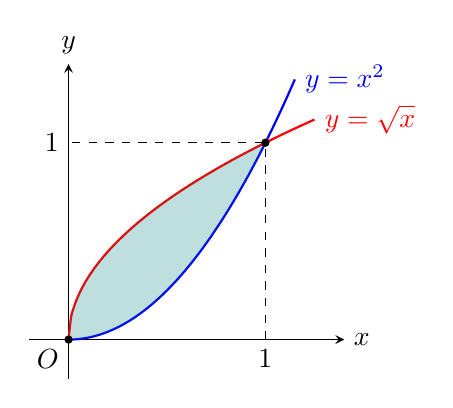
\begin{tikzpicture}[>=stealth, scale=2.5]
            \draw[->] (-0.2, 0) -- (1.4, 0) node[right] {$x$};
            \draw[->] (0, -0.2) -- (0, 1.4) node[above] {$y$};
            \node[below left] at (0, 0) {$O$};

            \draw[domain=0:1.15, samples=100, smooth, thick, blue] plot (\x, {\x*\x}) node[right] {$y = x^2$};
            \draw[domain=0:1.25, samples=100, smooth, thick, red] plot (\x, {sqrt(\x)}) node[right] {$y = \sqrt{x}$};
            \fill[teal, opacity=0.25, domain=0:1, samples=100]
            plot (\x, {sqrt(\x)}) -- plot[domain=1:0] (\x, {\x*\x}) -- cycle;

            \draw[dashed] (1, 0) node[below] {$1$} -- (1, 1) -- (0, 1) node[left] {$1$};
            \fill (0,0) circle (0.6pt);
            \fill (1,1) circle (0.6pt);
        \end{tikzpicture}
    \end{center}

    所围图形的面积为
    \begin{equation}
        S = \int_0^1 (\sqrt{x} - x^2) \d x = \left[ \frac{2}{3}x^{3/2} - \frac{1}{3}x^3 \right]_0^1 = \frac{2}{3} - \frac{1}{3} = \frac{1}{3}.
    \end{equation}
    \begin{equation}
        \boxed{S = \frac{1}{3}.}
    \end{equation}

    \ansitem{2}

    由图形关于 $y$ 轴的对称性，先考虑第一象限部分．

    \begin{center}
        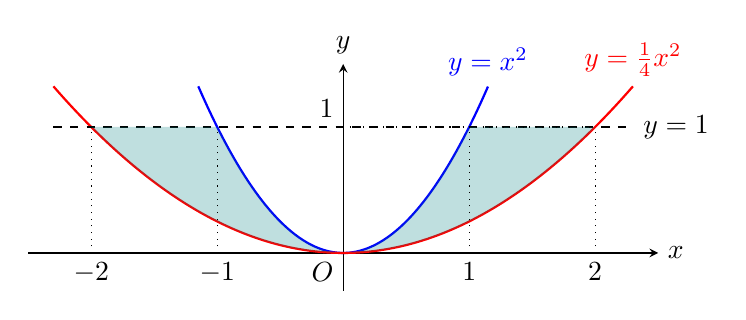
\begin{tikzpicture}[>=stealth, scale=1.6]
            \draw[->] (-2.5, 0) -- (2.5, 0) node[right] {$x$};
            \draw[->] (0, -0.3) -- (0, 1.5) node[above] {$y$};
            \node[below left] at (0, 0) {$O$};

            \draw[domain=-1.15:1.15, samples=100, smooth, thick, blue] plot (\x, {\x*\x}) node[above] {$y = x^2$};
            \draw[domain=-2.3:2.3, samples=100, smooth, thick, red] plot (\x, {0.25*\x*\x}) node[above] {$y = \frac{1}{4}x^2$};
            \draw[thick, dashed] (-2.3, 1) -- (2.3, 1) node[right] {$y = 1$};

            \fill[teal, opacity=0.25, domain=0:1, samples=100]
            plot (\x, {\x*\x}) -- (1,1) -- plot[domain=1:2] (\x, 1) -- plot[domain=2:0] (\x, {0.25*\x*\x}) -- cycle;
            \fill[teal, opacity=0.25, domain=-1:0, samples=100]
            plot (\x, {\x*\x}) -- (0,0) -- plot[domain=0:-2] (\x, {0.25*\x*\x}) -- plot[domain=-2:-1] (\x, 1) -- cycle;

            \draw[dotted] (1, 0) node[below] {$1$} -- (1, 1);
            \draw[dotted] (-1, 0) node[below] {$-1$} -- (-1, 1);
            \draw[dotted] (2, 0) node[below] {$2$} -- (2, 1);
            \draw[dotted] (-2, 0) node[below] {$-2$} -- (-2, 1);
            \draw[dotted] (0, 1) node[above left] {$1$} -- (2, 1);
        \end{tikzpicture}
    \end{center}

    将曲线方程改写为 $x$ 关于 $y$ 的函数：
    \begin{equation}
        x_1(y) = \sqrt{y}, \qquad x_2(y) = 2\sqrt{y} \quad (0 \leqslant y \leqslant 1).
    \end{equation}
    利用对 $y$ 的定积分计算全区域面积：
    \begin{equation}
        \begin{aligned}
            S & = 2 \int_0^1 \bigl( x_2(y) - x_1(y) \bigr) \d y          \\
              & = 2 \int_0^1 (2\sqrt{y} - \sqrt{y}) \d y                 \\
              & = 2 \int_0^1 \sqrt{y} \d y                               \\
              & = 2 \left[ \frac{2}{3}y^{3/2} \right]_0^1 = \frac{4}{3}.
        \end{aligned}
    \end{equation}
    \begin{equation}
        \boxed{S = \frac{4}{3}.}
    \end{equation}
\end{solution}

\begin{problem}{含有定积分的极限计算}{Limits-Involving-Definite-Integrals}
    求下列极限：
    \begin{enumerate}
        \item $\lim_{x\to 0} \frac{\int_0^x \sin t^3 \d t}{x^4}$；
        \item $\lim_{x\to 0} \frac{1}{\sin^3 x} \int_0^{\tan x} \arcsin t^2 \d t$；
        \item $\lim_{n\to\infty} \left[ \frac{1}{\sqrt{n^2}} + \frac{1}{\sqrt{n^2 - 1^2}} + \frac{1}{\sqrt{n^2 - 2^2}} + \cdots + \frac{1}{\sqrt{n^2 - (n-1)^2}} \right]$；
        \item $\lim_{n\to\infty} \frac{1^p + 2^p + \cdots + n^p}{n^{p+1}}$，$p$ 是常数，$p > 0$．
    \end{enumerate}
\end{problem}

\begin{solution}
    \ansitem{1}

    属于 $\frac{0}{0}$ 型未定式，应用 L'H\^{o}pital 法则：
    \begin{equation}
        \lim_{x\to 0} \frac{\int_0^x \sin t^3 \d t}{x^4} = \lim_{x\to 0} \frac{\sin x^3}{4x^3} = \frac{1}{4}.
    \end{equation}
    \begin{equation}
        \boxed{\lim_{x\to 0} \frac{\int_0^x \sin t^3 \d t}{x^4} = \frac{1}{4}.}
    \end{equation}

    \ansitem{2}

    因为当 $x \to 0$ 时 $\sin^3 x \sim x^3$，原式为 $\frac{0}{0}$ 型未定式，应用等价无穷小代换与 L'H\^{o}pital 法则：
    \begin{equation}
        \begin{aligned}
            \lim_{x\to 0} \frac{\int_0^{\tan x} \arcsin t^2 \d t}{\sin^3 x} & = \lim_{x\to 0} \frac{\int_0^{\tan x} \arcsin t^2 \d t}{x^3}    \\
                                                                            & = \lim_{x\to 0} \frac{\arcsin(\tan^2 x) \sec^2 x}{3x^2}         \\
                                                                            & = \frac{1}{3} \lim_{x\to 0} \frac{\tan^2 x}{x^2} = \frac{1}{3}.
        \end{aligned}
    \end{equation}
    \begin{equation}
        \boxed{\lim_{x\to 0} \frac{1}{\sin^3 x} \int_0^{\tan x} \arcsin t^2 \d t = \frac{1}{3}.}
    \end{equation}

    \ansitem{3}

    将和式变形为 Riemann 和的形式：
    \begin{equation}
        \sum_{k=0}^{n-1} \frac{1}{\sqrt{n^2 - k^2}}
        = \frac{1}{n}\sum_{k=0}^{n-1}
        \frac{1}{\sqrt{1 - \left(\frac{k}{n}\right)^2}}.
    \end{equation}

    令
    \begin{equation}
        h(x) = \frac{1}{\sqrt{1 - x^2}}, \qquad 0 \leqslant x < 1.
    \end{equation}
    函数 $h(x)$ 在 $[0, 1)$ 上连续且单调递增，并且在 $x = 1$ 处无界．因此这里不能直接将上述和式作为闭区间 $[0, 1]$ 上普通连续函数的 Riemann 和处理，而需对端点 $x = 1$ 单独进行估计．

    由于 $h(x)$ 在 $[0, 1)$ 上单调递增，对每个
    $k = 0, 1, \cdots, n - 1$，有
    \begin{equation}
        \frac{1}{n}h\left(\frac{k}{n}\right)
        \leqslant
        \int_{\frac{k}{n}}^{\frac{k+1}{n}} h(x)\d x.
    \end{equation}
    对 $k$ 求和，得
    \begin{equation}
        \frac{1}{n}\sum_{k=0}^{n-1}h\left(\frac{k}{n}\right)
        \leqslant
        \int_0^1 h(x)\d x.
    \end{equation}
    因此
    \begin{equation}
        \limsup_{n\to\infty}
        \frac{1}{n}\sum_{k=0}^{n-1}h\left(\frac{k}{n}\right)
        \leqslant
        \int_0^1 \frac{1}{\sqrt{1-x^2}}\d x
        = \frac{\uppi}{2}.
    \end{equation}

    另一方面，任取 $r \in (0, 1)$，令
    \begin{equation}
        m_n = \lfloor nr \rfloor.
    \end{equation}
    由于各项均为正数，有
    \begin{equation}
        \frac{1}{n}\sum_{k=0}^{n-1}h\left(\frac{k}{n}\right)
        \geqslant
        \frac{1}{n}\sum_{k=0}^{m_n-1}h\left(\frac{k}{n}\right).
    \end{equation}
    因为 $h(x)$ 在闭区间 $[0, r]$ 上连续，且
    $\frac{m_n}{n}\to r$，由 Riemann 和的定义可得
    \begin{equation}
        \lim_{n\to\infty}
        \frac{1}{n}\sum_{k=0}^{m_n-1}h\left(\frac{k}{n}\right)
        =
        \int_0^r h(x)\d x.
    \end{equation}
    从而
    \begin{equation}
        \liminf_{n\to\infty}
        \frac{1}{n}\sum_{k=0}^{n-1}h\left(\frac{k}{n}\right)
        \geqslant
        \int_0^r \frac{1}{\sqrt{1-x^2}}\d x
        = \arcsin r.
    \end{equation}
    令 $r\to1^-$，得到
    \begin{equation}
        \liminf_{n\to\infty}
        \frac{1}{n}\sum_{k=0}^{n-1}h\left(\frac{k}{n}\right)
        \geqslant
        \lim_{r\to1^-}\arcsin r
        = \frac{\uppi}{2}.
    \end{equation}

    综合上、下极限的估计：
    \begin{equation}
        \limsup_{n\to\infty}
        \frac{1}{n}\sum_{k=0}^{n-1}h\left(\frac{k}{n}\right)
        \leqslant \frac{\uppi}{2}
        \leqslant
        \liminf_{n\to\infty}
        \frac{1}{n}\sum_{k=0}^{n-1}h\left(\frac{k}{n}\right).
    \end{equation}
    因此极限存在且等于 $\frac{\uppi}{2}$，即
    \begin{equation}
        \boxed{
            \lim_{n\to\infty}
            \left[
                \frac{1}{\sqrt{n^2}}
                + \frac{1}{\sqrt{n^2 - 1^2}}
                + \cdots
                + \frac{1}{\sqrt{n^2 - (n-1)^2}}
                \right]
            = \frac{\uppi}{2}.
        }
    \end{equation}

    \ansitem{4}

    将和式提取因子 $\frac{1}{n}$：
    \begin{equation}
        \frac{1^p + 2^p + \cdots + n^p}{n^{p+1}} = \frac{1}{n}\sum_{k=1}^n \left( \frac{k}{n} \right)^p.
    \end{equation}
    由定积分的定义：
    \begin{equation}
        \lim_{n\to\infty} \frac{1}{n}\sum_{k=1}^n \left( \frac{k}{n} \right)^p = \int_0^1 x^p \d x = \left[ \frac{x^{p+1}}{p+1} \right]_0^1 = \frac{1}{p+1}.
    \end{equation}
    \begin{equation}
        \boxed{\lim_{n\to\infty} \frac{1^p + 2^p + \cdots + n^p}{n^{p+1}} = \frac{1}{p+1}.}
    \end{equation}
\end{solution}

\begin{problem}{含参定积分的极限计算}{Limits-Of-Parametric-Integrals}
    求下列极限：
    \begin{enumerate}
        \item $\lim_{n\to\infty} \int_a^b \e^{-nx^2} \d x$，这里 $a, b$ 为常数，且 $0 < a < b$；
        \item $\lim_{n\to\infty} \int_0^1 \frac{x^n}{1 + x} \d x$；
        \item $\lim_{n\to\infty} \int_n^{n+a} \frac{\sin x}{x} \d x$，这里 $a$ 为常数，且 $a > 0$．
    \end{enumerate}
    （注意：对于 (2) 若用积分中值定理，所说的积分为 $\frac{\xi^n}{1+\xi}$，其中 $0 < \xi < 1$；但这时 $\xi$ 与 $n$ 有关，故在 $n\to\infty$ 时，不能断言 $\xi^n \to 0$．）
\end{problem}

\begin{solution}
    \ansitem{1}

    当 $x \in [a, b]$（$0 < a < b$）时，恒有 $x^2 \geqslant a^2 > 0$，从而
    \begin{equation}
        0 < \e^{-nx^2} \leqslant \e^{-na^2}.
    \end{equation}
    两边在 $[a, b]$ 上积分得
    \begin{equation}
        0 < \int_a^b \e^{-nx^2} \d x \leqslant (b - a)\e^{-na^2}.
    \end{equation}
    因为 $\lim_{n\to\infty} (b - a)\e^{-na^2} = 0$，由夹逼准则可得
    \begin{equation}
        \boxed{\lim_{n\to\infty} \int_a^b \e^{-nx^2} \d x = 0.}
    \end{equation}

    \ansitem{2}

    当 $x \in [0, 1]$ 时，恒有 $1 \leqslant 1 + x \leqslant 2 \implies \frac{1}{2} \leqslant \frac{1}{1+x} \leqslant 1$，从而
    \begin{equation}
        \frac{1}{2}x^n \leqslant \frac{x^n}{1 + x} \leqslant x^n.
    \end{equation}
    两端在 $[0, 1]$ 上积分得
    \begin{equation}
        \frac{1}{2(n + 1)} \leqslant \int_0^1 \frac{x^n}{1 + x} \d x \leqslant \frac{1}{n + 1}.
    \end{equation}
    因为 $\lim_{n\to\infty} \frac{1}{2(n+1)} = \lim_{n\to\infty} \frac{1}{n+1} = 0$，由夹逼准则可得
    \begin{equation}
        \boxed{\lim_{n\to\infty} \int_0^1 \frac{x^n}{1 + x} \d x = 0.}
    \end{equation}

    \ansitem{3}

    当 $x \in [n, n + a]$（$n > 0, a > 0$）时，有
    \begin{equation}
        \left| \frac{\sin x}{x} \right| \leqslant \frac{1}{x} \leqslant \frac{1}{n}.
    \end{equation}
    利用定积分绝对值不等式估计：
    \begin{equation}
        0 \leqslant \left| \int_n^{n+a} \frac{\sin x}{x} \d x \right| \leqslant \int_n^{n+a} \left| \frac{\sin x}{x} \right| \d x \leqslant \int_n^{n+a} \frac{1}{n} \d x = \frac{a}{n}.
    \end{equation}
    因为 $\lim_{n\to\infty} \frac{a}{n} = 0$，由夹逼准则可得
    \begin{equation}
        \boxed{\lim_{n\to\infty} \int_n^{n+a} \frac{\sin x}{x} \d x = 0.}
    \end{equation}
\end{solution}

\begin{problem}{对称区间上奇偶函数的定积分性质}{Definite-Integrals-Of-Odd-And-Even-Functions}
    设函数 $f(x)$ 在区间 $[-a, a]$ 上连续．证明：
    \begin{enumerate}
        \item 若 $f(x)$ 是奇函数，则 $\int_{-a}^a f(x) \d x = 0$；
        \item 若 $f(x)$ 是偶函数，则 $\int_{-a}^a f(x) \d x = 2\int_0^a f(x) \d x$．
    \end{enumerate}
\end{problem}

\begin{myproof}
    将对称区间 $[-a, a]$ 上的积分拆分为两部分：
    \begin{equation}
        \int_{-a}^a f(x) \d x = \int_{-a}^0 f(x) \d x + \int_0^a f(x) \d x.
    \end{equation}
    对第一项作换元 $x = -t$，则 $\d x = -\d t$，上下限分别变为 $a$ 与 $0$：
    \begin{equation}
        \int_{-a}^0 f(x) \d x = \int_a^0 f(-t) (-\d t) = \int_0^a f(-t) \d t = \int_0^a f(-x) \d x.
    \end{equation}
    代回原式可得
    \begin{equation}
        \int_{-a}^a f(x) \d x = \int_0^a \bigl( f(-x) + f(x) \bigr) \d x.
    \end{equation}

    \ansitem{1}

    若 $f(x)$ 为奇函数，则对任意 $x$ 恒有 $f(-x) = -f(x)$，故 $f(-x) + f(x) = 0$：
    \begin{equation}
        \int_{-a}^a f(x) \d x = \int_0^a 0 \d x = 0.
    \end{equation}

    \ansitem{2}

    若 $f(x)$ 为偶函数，则对任意 $x$ 恒有 $f(-x) = f(x)$，故 $f(-x) + f(x) = 2f(x)$：
    \begin{equation}
        \int_{-a}^a f(x) \d x = \int_0^a 2f(x) \d x = 2\int_0^a f(x) \d x.
    \end{equation}
\end{myproof}

\begin{problem}{周期函数定积分的平移不变性}{Translation-Invariance-Of-Periodic-Integrals}
    设 $f(x)$ 为具有周期 $T$ 的连续函数，证明：对任意的常数 $a$，有
    \begin{equation}
        \int_a^{a+T} f(x) \d x = \int_0^T f(x) \d x.
    \end{equation}
\end{problem}

\begin{myproof}
    设函数
    \begin{equation}
        I(a) = \int_a^{a+T} f(x) \d x = \int_0^{a+T} f(x) \d x - \int_0^a f(x) \d x.
    \end{equation}
    因为 $f(x)$ 为连续函数，应用变上限积分求导法则对 $a$ 求导：
    \begin{equation}
        I'(a) = f(a + T) \cdot (a + T)' - f(a) \cdot (a)' = f(a + T) - f(a).
    \end{equation}
    由于 $f(x)$ 是以 $T$ 为周期的函数，对一切实数 $a$ 恒有 $f(a + T) = f(a)$，因此
    \begin{equation}
        I'(a) = 0.
    \end{equation}
    导数恒为零表明函数 $I(a)$ 为常数函数，即对任意常数 $a$，恒有
    \begin{equation}
        I(a) = I(0),
    \end{equation}
    即
    \begin{equation}
        \int_a^{a+T} f(x) \d x = \int_0^T f(x) \d x.
    \end{equation}
\end{myproof}

\begin{problem}{定积分的综合计算}{Definite-Integrals-Comprehensive-Calculation}
    计算下列积分：
    \begin{enumerate}
        \item $\int_0^{2\uppi} |\cos x| \d x$；
        \item $\int_{-3}^4 [x] \d x$；
        \item $\int_{-1}^1 \cos x \ln\frac{1 + x}{1 - x} \d x$；
        \item $\int_{-\frac{\uppi}{2}}^{\frac{\uppi}{2}} \frac{1}{1 + \e^x} \cos^3 x \d x$；
        \item $\int_0^{\ln 2} \sqrt{1 - \e^{-2x}} \d x$；
        \item $\int_0^1 x \arcsin x \d x$；
        \item $\int_0^1 x^3 \e^x \d x$；
        \item $\int_0^a \frac{1}{x + \sqrt{a^2 - x^2}} \d x$；
        \item $\int_0^{\frac{\uppi}{4}} \sqrt{\tan x} \d x$；
        \item $\int_0^{\frac{\uppi}{2}} \frac{1}{a^2 \sin^2 x + b^2 \cos^2 x} \d x$（$a > 0, b > 0$）；
        \item $\int_{-1}^1 x^4 \sqrt{1 - x^2} \d x$；
        \item $\int_0^{2\uppi} \sin^6 x \d x$；
        \item $\int_{-1}^1 \e^{|x|} \cdot \arctan \e^x \d x$；
        \item $\int_0^{\uppi} \frac{\sec^2 x}{2 + \tan^2 x} \d x$．
    \end{enumerate}
\end{problem}

\begin{solution}
    \ansitem{1}

    利用周期性与对称性：
    \begin{equation}
        \int_0^{2\uppi} |\cos x| \d x = 4 \int_0^{\frac{\uppi}{2}} \cos x \d x = 4 [\sin x]_0^{\frac{\uppi}{2}} = 4.
    \end{equation}
    \begin{equation}
        \boxed{\int_0^{2\uppi} |\cos x| \d x = 4.}
    \end{equation}

    \ansitem{2}

    分区间计算阶梯函数的积分：
    \begin{equation}
        \int_{-3}^4 [x] \d x = \sum_{k=-3}^3 \int_k^{k+1} k \d x = \sum_{k=-3}^3 k = -3 - 2 - 1 + 0 + 1 + 2 + 3 = 0.
    \end{equation}
    \begin{equation}
        \boxed{\int_{-3}^4 [x] \d x = 0.}
    \end{equation}

    \ansitem{3}

    设被积函数为 $g(x) = \cos x \ln\frac{1 + x}{1 - x}$．因为
    \begin{equation}
        g(-x) = \cos(-x) \ln\frac{1 - x}{1 + x} = -\cos x \ln\frac{1 + x}{1 - x} = -g(x),
    \end{equation}
    即 $g(x)$ 为对称区间 $[-1, 1]$ 上的奇函数，故
    \begin{equation}
        \int_{-1}^1 \cos x \ln\frac{1 + x}{1 - x} \d x = 0.
    \end{equation}
    \begin{equation}
        \boxed{\int_{-1}^1 \cos x \ln\frac{1 + x}{1 - x} \d x = 0.}
    \end{equation}

    \ansitem{4}

    设 $I = \int_{-\frac{\uppi}{2}}^{\frac{\uppi}{2}} \frac{\cos^3 x}{1 + \e^x} \d x$．作代换 $x = -t$：
    \begin{equation}
        I = \int_{-\frac{\uppi}{2}}^{\frac{\uppi}{2}} \frac{\cos^3(-t)}{1 + \e^{-t}} \d t = \int_{-\frac{\uppi}{2}}^{\frac{\uppi}{2}} \frac{\e^x \cos^3 x}{1 + \e^x} \d x.
    \end{equation}
    两式相加得
    \begin{equation}
        2I = \int_{-\frac{\uppi}{2}}^{\frac{\uppi}{2}} \frac{1 + \e^x}{1 + \e^x}\cos^3 x \d x = \int_{-\frac{\uppi}{2}}^{\frac{\uppi}{2}} \cos^3 x \d x = 2\int_0^{\frac{\uppi}{2}} \cos^3 x \d x = 2 \cdot \frac{2}{3} = \frac{4}{3}.
    \end{equation}
    因此 $I = \frac{2}{3}$．
    \begin{equation}
        \boxed{\int_{-\frac{\uppi}{2}}^{\frac{\uppi}{2}} \frac{1}{1 + \e^x} \cos^3 x \d x = \frac{2}{3}.}
    \end{equation}

    \ansitem{5}

    令 $t = \sqrt{1 - \e^{-2x}}$，则 $\e^{-2x} = 1 - t^2$，$x = -\frac{1}{2}\ln(1 - t^2)$，$\d x = \frac{t}{1 - t^2}\d t$：
    \begin{equation}
        \begin{aligned}
            \int_0^{\ln 2} \sqrt{1 - \e^{-2x}} \d x & = \int_0^{\frac{\sqrt{3}}{2}} \frac{t^2}{1 - t^2} \d t = \int_0^{\frac{\sqrt{3}}{2}} \left( -1 + \frac{1}{1 - t^2} \right) \d t \\
                                                    & = \left[ -t + \frac{1}{2}\ln\left( \frac{1 + t}{1 - t} \right) \right]_0^{\frac{\sqrt{3}}{2}}                                   \\
                                                    & = -\frac{\sqrt{3}}{2} + \frac{1}{2}\ln(7 + 4\sqrt{3})                                                                           \\
                                                    & = \ln(2 + \sqrt{3}) - \frac{\sqrt{3}}{2}.
        \end{aligned}
    \end{equation}
    \begin{equation}
        \boxed{\int_0^{\ln 2} \sqrt{1 - \e^{-2x}} \d x = \ln(2 + \sqrt{3}) - \frac{\sqrt{3}}{2}.}
    \end{equation}

    \ansitem{6}

    应用分部积分法：
    \begin{equation}
        \begin{aligned}
            \int_0^1 x \arcsin x \d x & = \left[ \frac{2x^2 - 1}{4}\arcsin x + \frac{x\sqrt{1 - x^2}}{4} \right]_0^1  \\
                                      & = \left( \frac{1}{4} \cdot \frac{\uppi}{2} + 0 \right) - 0 = \frac{\uppi}{8}.
        \end{aligned}
    \end{equation}
    \begin{equation}
        \boxed{\int_0^1 x \arcsin x \d x = \frac{\uppi}{8}.}
    \end{equation}

    \ansitem{7}

    连续应用分部积分法：
    \begin{equation}
        \int_0^1 x^3 \e^x \d x = \left[ (x^3 - 3x^2 + 6x - 6)\e^x \right]_0^1 = -2\e - (-6) = 6 - 2\e.
    \end{equation}
    \begin{equation}
        \boxed{\int_0^1 x^3 \e^x \d x = 6 - 2\e.}
    \end{equation}

    \ansitem{8}

    令 $x = a \sin t$（$t \in \left[0, \frac{\uppi}{2}\right]$），$\d x = a\cos t \d t$：
    \begin{equation}
        \int_0^a \frac{1}{x + \sqrt{a^2 - x^2}} \d x = \int_0^{\frac{\uppi}{2}} \frac{a\cos t}{a\sin t + a\cos t} \d t = \int_0^{\frac{\uppi}{2}} \frac{\cos t}{\sin t + \cos t} \d t = \frac{\uppi}{4}.
    \end{equation}
    \begin{equation}
        \boxed{\int_0^a \frac{1}{x + \sqrt{a^2 - x^2}} \d x = \frac{\uppi}{4}.}
    \end{equation}

    \ansitem{9}

    令 $t = \sqrt{\tan x}$，则 $\d x = \frac{2t}{1 + t^4}\d t$：
    \begin{equation}
        \begin{aligned}
            \int_0^{\frac{\uppi}{4}} \sqrt{\tan x} \d x & = \int_0^1 \frac{2t^2}{1 + t^4} \d t                                                                                                                                          \\
                                                        & = \left[ \frac{1}{\sqrt{2}}\arctan\left( \frac{t^2 - 1}{\sqrt{2}t} \right) + \frac{1}{2\sqrt{2}}\ln\left( \frac{t^2 - \sqrt{2}t + 1}{t^2 + \sqrt{2}t + 1} \right) \right]_0^1 \\
                                                        & = \frac{\sqrt{2}\uppi}{4} + \frac{\sqrt{2}}{2}\ln(\sqrt{2} - 1).
        \end{aligned}
    \end{equation}
    \begin{equation}
        \boxed{\int_0^{\frac{\uppi}{4}} \sqrt{\tan x} \d x = \frac{\sqrt{2}\uppi}{4} + \frac{\sqrt{2}}{2}\ln(\sqrt{2} - 1).}
    \end{equation}

    \ansitem{10}

    分子分母同除以 $\cos^2 x$：
    \begin{equation}
        \begin{aligned}
            \int_0^{\frac{\uppi}{2}} \frac{1}{a^2 \sin^2 x + b^2 \cos^2 x} \d x & = \int_0^{+\infty} \frac{\d(\tan x)}{a^2 \tan^2 x + b^2}                                              \\
                                                                                & = \left[ \frac{1}{ab}\arctan\left( \frac{a\tan x}{b} \right) \right]_0^{+\infty} = \frac{\uppi}{2ab}.
        \end{aligned}
    \end{equation}
    \begin{equation}
        \boxed{\int_0^{\frac{\uppi}{2}} \frac{1}{a^2 \sin^2 x + b^2 \cos^2 x} \d x = \frac{\uppi}{2ab}.}
    \end{equation}

    \ansitem{11}

    利用被积函数的偶函数性质，令 $x = \sin t$ 并应用 Wallis 公式：
    \begin{equation}
        \begin{aligned}
            \int_{-1}^1 x^4 \sqrt{1 - x^2} \d x & = 2\int_0^1 x^4 \sqrt{1 - x^2} \d x = 2\int_0^{\frac{\uppi}{2}} \sin^4 t \cos^2 t \d t                                             \\
                                                & = 2\int_0^{\frac{\uppi}{2}} (\sin^4 t - \sin^6 t) \d t = 2\left( \frac{3\uppi}{16} - \frac{5\uppi}{32} \right) = \frac{\uppi}{16}.
        \end{aligned}
    \end{equation}
    \begin{equation}
        \boxed{\int_{-1}^1 x^4 \sqrt{1 - x^2} \d x = \frac{\uppi}{16}.}
    \end{equation}

    \ansitem{12}

    利用正弦函数的高次周期性与 Wallis 公式：
    \begin{equation}
        \int_0^{2\uppi} \sin^6 x \d x = 4\int_0^{\frac{\uppi}{2}} \sin^6 x \d x = 4 \cdot \frac{5 \cdot 3 \cdot 1}{6 \cdot 4 \cdot 2} \cdot \frac{\uppi}{2} = \frac{5\uppi}{8}.
    \end{equation}
    \begin{equation}
        \boxed{\int_0^{2\uppi} \sin^6 x \d x = \frac{5\uppi}{8}.}
    \end{equation}

    \ansitem{13}

    设 $I = \int_{-1}^1 \e^{|x|}\arctan \e^x \d x$．作代换 $x = -t$：
    \begin{equation}
        I = \int_{-1}^1 \e^{|t|}\arctan(\e^{-t})\d t = \int_{-1}^1 \e^{|x|}\arctan\left( \frac{1}{\e^x} \right)\d x.
    \end{equation}
    利用恒等式 $\arctan u + \arctan\frac{1}{u} = \frac{\uppi}{2}$（$u > 0$）：
    \begin{equation}
        2I = \frac{\uppi}{2}\int_{-1}^1 \e^{|x|}\d x = \uppi \int_0^1 \e^x \d x = \uppi(\e - 1) \implies I = \frac{\uppi(\e - 1)}{2}.
    \end{equation}
    \begin{equation}
        \boxed{\int_{-1}^1 \e^{|x|} \cdot \arctan \e^x \d x = \frac{\uppi(\e - 1)}{2}.}
    \end{equation}

    \ansitem{14}

    以 $x = \frac{\uppi}{2}$ 为奇点拆分反常积分：
    \begin{equation}
        \begin{aligned}
            \int_0^{\uppi} \frac{\sec^2 x}{2 + \tan^2 x} \d x & = \int_0^{\frac{\uppi}{2}} \frac{\sec^2 x}{2 + \tan^2 x} \d x + \int_{\frac{\uppi}{2}}^{\uppi} \frac{\sec^2 x}{2 + \tan^2 x} \d x \\
                                                              & = \int_0^{+\infty} \frac{\d u}{2 + u^2} + \int_{-\infty}^0 \frac{\d u}{2 + u^2}                                                   \\
                                                              & = \frac{\uppi}{2\sqrt{2}} + \frac{\uppi}{2\sqrt{2}} = \frac{\sqrt{2}\uppi}{2}.
        \end{aligned}
    \end{equation}
    \begin{equation}
        \boxed{\int_0^{\uppi} \frac{\sec^2 x}{2 + \tan^2 x} \d x = \frac{\sqrt{2}\uppi}{2}.}
    \end{equation}
\end{solution}

\begin{problem}{对称积分恒等式及其应用}{Symmetric-Integral-Identity-And-Application}
    设 $f(x)$ 在 $[0, 1]$ 上连续，证明：
    \begin{equation}
        \int_0^{\uppi} x f(\sin x) \d x = \uppi \int_0^{\frac{\uppi}{2}} f(\sin x) \d x;
    \end{equation}
    并用这一结果计算 $\int_0^{\uppi} \frac{x\sin x}{1 + \cos^2 x} \d x$．
\end{problem}

\begin{solution}
    令 $x = \uppi - t$，$\d x = -\d t$：
    \begin{equation}
        \begin{aligned}
            \int_0^{\uppi} x f(\sin x) \d x & = \int_0^{\uppi} (\uppi - t) f\bigl(\sin(\uppi - t)\bigr) \d t           \\
                                            & = \uppi \int_0^{\uppi} f(\sin t) \d t - \int_0^{\uppi} t f(\sin t) \d t.
        \end{aligned}
    \end{equation}
    移项整理得
    \begin{equation}
        \int_0^{\uppi} x f(\sin x) \d x = \frac{\uppi}{2} \int_0^{\uppi} f(\sin x) \d x.
    \end{equation}
    又因为 $f(\sin(\uppi - x)) = f(\sin x)$，图形关于 $x = \frac{\uppi}{2}$ 对称，所以
    \begin{equation}
        \int_0^{\uppi} f(\sin x) \d x = 2\int_0^{\frac{\uppi}{2}} f(\sin x) \d x \implies \int_0^{\uppi} x f(\sin x) \d x = \uppi \int_0^{\frac{\uppi}{2}} f(\sin x) \d x.
    \end{equation}
    将原积分化为应用上述公式的形式：
    \begin{equation}
        \begin{aligned}
            \int_0^{\uppi} \frac{x\sin x}{1 + \cos^2 x} \d x & = \int_0^{\uppi} x \cdot \frac{\sin x}{2 - \sin^2 x} \d x = \uppi \int_0^{\frac{\uppi}{2}} \frac{\sin x}{1 + \cos^2 x} \d x \\
                                                             & = \uppi \int_0^{\frac{\uppi}{2}} \frac{-\d(\cos x)}{1 + \cos^2 x} = \uppi [-\arctan(\cos x)]_0^{\frac{\uppi}{2}}            \\
                                                             & = \uppi \left( 0 - \left(-\frac{\uppi}{4}\right) \right) = \frac{\uppi^2}{4}.
        \end{aligned}
    \end{equation}
    \begin{equation}
        \boxed{\int_0^{\uppi} \frac{x\sin x}{1 + \cos^2 x} \d x = \frac{\uppi^2}{4}.}
    \end{equation}
\end{solution}

\begin{problem}{非初等原函数定积分的放缩不等式}{Inequality-Estimation-For-Non-Elementary-Integral}
    证明：$\frac{1}{6} < \int_0^1 \sin x^2 \d x < \frac{1}{3}$．（注意：本题中被积函数 $\sin x^2$ 虽然可积，但其原函数是不能用初等函数表示的．因此试图通过求问题中的积分是徒劳的）．
\end{problem}

\begin{myproof}
    对任意 $t \in (0, 1)$，利用正弦函数的 Taylor 展开式及交错级数性质，恒有不等式
    \begin{equation}
        t - \frac{t^3}{6} < \sin t < t.
    \end{equation}
    令 $t = x^2$，当 $x \in (0, 1)$ 时，代入上式得
    \begin{equation}
        x^2 - \frac{x^6}{6} < \sin x^2 < x^2.
    \end{equation}
    在闭区间 $[0, 1]$ 上逐项取定积分：
    \begin{equation}
        \int_0^1 \left( x^2 - \frac{x^6}{6} \right) \d x < \int_0^1 \sin x^2 \d x < \int_0^1 x^2 \d x.
    \end{equation}
    分别计算左、右端定积分值：
    \begin{equation}
        \int_0^1 x^2 \d x = \left[ \frac{x^3}{3} \right]_0^1 = \frac{1}{3},
    \end{equation}
    \begin{equation}
        \int_0^1 \left( x^2 - \frac{x^6}{6} \right) \d x = \left[ \frac{x^3}{3} - \frac{x^7}{42} \right]_0^1 = \frac{1}{3} - \frac{1}{42} = \frac{13}{42}.
    \end{equation}
    因为 $\frac{13}{42} > \frac{7}{42} = \frac{1}{6}$，所以
    \begin{equation}
        \frac{1}{6} < \frac{13}{42} < \int_0^1 \sin x^2 \d x < \frac{1}{3}.
    \end{equation}
    即证
    \begin{equation}
        \frac{1}{6} < \int_0^1 \sin x^2 \d x < \frac{1}{3}.
    \end{equation}
\end{myproof}

\begin{problem}{函数的平均值与最值计算}{Average-And-Extremum-Of-Functions}
    设函数 $f(x)$ 在 $[a, b]$ 上可积，我们将 $\frac{1}{b-a}\int_a^b f(x) \d x$ 定义为函数 $f(x)$ 在区间 $[a, b]$ 上的平均值．对下列函数，计算在指定区间上的平均值，以及最大、最小值：
    \begin{enumerate}
        \item $f(x) = x$，区间为 $[0, 1]$ 及 $[0, 10^5]$；
        \item $f(x) = \e^{-x}$，区间为 $[0, 1]$ 及 $[0, 10^5]$；
        \item $f(x) = x\e^{-x}$，区间为 $[0, 1]$ 及 $[0, 10^5]$．
    \end{enumerate}
\end{problem}

\begin{solution}
    \ansitem{1}

    函数 $f(x) = x$ 在 $\symbb{R}$ 上严格单调递增：
    \begin{enumerate}
        \item 在区间 $[0, 1]$ 上：
              \begin{equation}
                  \bar{f} = \frac{1}{1 - 0}\int_0^1 x \d x = \left[ \frac{1}{2}x^2 \right]_0^1 = \frac{1}{2},
              \end{equation}
              最小值为 $\min_{x\in [0, 1]} f(x) = f(0) = 0$，最大值为 $\max_{x\in [0, 1]} f(x) = f(1) = 1$．
        \item 在区间 $[0, 10^5]$ 上：
              \begin{equation}
                  \bar{f} = \frac{1}{10^5}\int_0^{10^5} x \d x = \frac{1}{10^5} \left[ \frac{1}{2}x^2 \right]_0^{10^5} = \frac{10^5}{2} = 50000,
              \end{equation}
              最小值为 $\min_{x\in [0, 10^5]} f(x) = f(0) = 0$，最大值为 $\max_{x\in [0, 10^5]} f(x) = f(10^5) = 10^5$．
    \end{enumerate}
    \begin{equation}
        \boxed{\begin{aligned}
                 & [0, 1]: \bar{f} = \frac{1}{2}, \quad \min = 0, \quad \max = 1; \\
                 & [0, 10^5]: \bar{f} = 50000, \quad \min = 0, \quad \max = 10^5.
            \end{aligned}}
    \end{equation}

    \ansitem{2}

    函数 $f(x) = \e^{-x}$ 在 $\symbb{R}$ 上严格单调递减：
    \begin{enumerate}
        \item 在区间 $[0, 1]$ 上：
              \begin{equation}
                  \bar{f} = \frac{1}{1 - 0}\int_0^1 \e^{-x} \d x = [-\e^{-x}]_0^1 = 1 - \e^{-1},
              \end{equation}
              最小值为 $\min_{x\in [0, 1]} f(x) = f(1) = \e^{-1}$，最大值为 $\max_{x\in [0, 1]} f(x) = f(0) = 1$．
        \item 在区间 $[0, 10^5]$ 上：
              \begin{equation}
                  \bar{f} = \frac{1}{10^5}\int_0^{10^5} \e^{-x} \d x = \frac{1 - \e^{-10^5}}{10^5},
              \end{equation}
              最小值为 $\min_{x\in [0, 10^5]} f(x) = f(10^5) = \e^{-10^5}$，最大值为 $\max_{x\in [0, 10^5]} f(x) = f(0) = 1$．
    \end{enumerate}
    \begin{equation}
        \boxed{\begin{aligned}
                 & [0, 1]: \bar{f} = 1 - \e^{-1}, \quad \min = \e^{-1}, \quad \max = 1;                       \\
                 & [0, 10^5]: \bar{f} = \frac{1 - \e^{-10^5}}{10^5}, \quad \min = \e^{-10^5}, \quad \max = 1.
            \end{aligned}}
    \end{equation}

    \ansitem{3}

    对 $f(x) = x\e^{-x}$ 求导，得 $f'(x) = (1 - x)\e^{-x}$．因此 $f(x)$ 在 $[0, 1]$ 上单调递增，在 $[1, +\infty)$ 上单调递减：
    \begin{enumerate}
        \item 在区间 $[0, 1]$ 上：
              \begin{equation}
                  \bar{f} = \frac{1}{1 - 0}\int_0^1 x\e^{-x} \d x = [-(x + 1)\e^{-x}]_0^1 = 1 - 2\e^{-1},
              \end{equation}
              最小值为 $\min_{x\in [0, 1]} f(x) = f(0) = 0$，最大值为 $\max_{x\in [0, 1]} f(x) = f(1) = \e^{-1}$．
        \item 在区间 $[0, 10^5]$ 上：
              \begin{equation}
                  \bar{f} = \frac{1}{10^5}\int_0^{10^5} x\e^{-x} \d x = \frac{1 - (10^5 + 1)\e^{-10^5}}{10^5},
              \end{equation}
              最小值为 $\min_{x\in [0, 10^5]} f(x) = f(0) = 0$（因为 $f(10^5) = 10^5 \e^{-10^5} > 0$），最大值为 $\max_{x\in [0, 10^5]} f(x) = f(1) = \e^{-1}$．
    \end{enumerate}
    \begin{equation}
        \boxed{\begin{aligned}
                 & [0, 1]: \bar{f} = 1 - 2\e^{-1}, \quad \min = 0, \quad \max = \e^{-1};                             \\
                 & [0, 10^5]: \bar{f} = \frac{1 - (10^5 + 1)\e^{-10^5}}{10^5}, \quad \min = 0, \quad \max = \e^{-1}.
            \end{aligned}}
    \end{equation}
\end{solution}

\begin{problem}{定积分的估计与近似计算}{Integral-Estimation-And-Approximation}
    考虑积分 $I = \int_0^{100} \frac{\e^{-x}}{x + 100} \d x$．
    \begin{enumerate}
        \item 试给出 $I$ 的尽可能好的上、下界估计；
        \item 求出 $I$ 的近似值，精确到 $0.0001$．
    \end{enumerate}
\end{problem}

\begin{solution}
    \ansitem{1}

    当 $x \in [0, 100]$ 时，利用不等式
    \begin{equation}
        \frac{1}{100} - \frac{x}{100^2} < \frac{1}{x + 100} < \frac{1}{100} - \frac{x}{100^2} + \frac{x^2}{100^3}.
    \end{equation}
    两端同乘 $\e^{-x} > 0$ 并在区间 $[0, 100]$ 上积分：
    \begin{equation}
        \int_0^{100} \e^{-x}\left( \frac{1}{100} - \frac{x}{100^2} \right) \d x < I < \int_0^{100} \e^{-x}\left( \frac{1}{100} - \frac{x}{100^2} + \frac{x^2}{100^3} \right) \d x.
    \end{equation}
    计算各项积分（注意到 $\e^{-100} < 10^{-43}$ 可忽略）：
    \begin{equation}
        \int_0^{100} \e^{-x} \d x = 1 - \e^{-100}, \qquad \int_0^{100} x\e^{-x} \d x = 1 - 101\e^{-100},
    \end{equation}
    \begin{equation}
        \int_0^{100} x^2\e^{-x} \d x = 2 - (100^2 + 200 + 2)\e^{-100}.
    \end{equation}
    代入可得精确的上、下界估计：
    \begin{equation}
        0.0099 < \frac{99 + \e^{-100}}{10000} < I < \frac{99}{10000} + \frac{2}{10^6} = 0.009902.
    \end{equation}
    \begin{equation}
        \boxed{0.0099 < I < 0.009902.}
    \end{equation}

    \ansitem{2}

    由 (1) 的高精度上、下界估计：
    \begin{equation}
        0.009900 < I < 0.009902.
    \end{equation}
    精确到 $0.0001$ 时，其近似值为 $0.0099$．
    \begin{equation}
        \boxed{I \approx 0.0099.}
    \end{equation}
\end{solution}

\begin{problem}{单调函数定积分不等式的证明}{Monotone-Function-Integral-Inequality}
    \begin{enumerate}
        \item 设 $f(x)$ 是 $[0, 1]$ 上单调递减的连续函数．证明：对任意 $\alpha \in (0, 1)$，有
              \begin{equation}
                  \int_0^\alpha f(x) \d x \geqslant \alpha \int_0^1 f(x) \d x.
              \end{equation}
        \item 若仅假设 $f(x)$ 在 $[0, 1]$ 上单调递减，证明同样的结论．
    \end{enumerate}
    提示：(1) 有几种证法．第一种方法：利用 $\int_0^\alpha f(x) \d x = \alpha \int_0^1 f(\alpha x) \d x$；第二种方法：考虑 $g(\alpha) = \frac{1}{\alpha}\int_0^\alpha f(x) \d x$ ($0 < \alpha < 1$)，证明 $g(\alpha)$ 是单调递减函数．但是，这两种方法都需要 $f(x)$ 连续这一假设，因此都不适用于解决 (2)．
\end{problem}

\begin{solution}
    \ansitem{1}

    采用第一种变量代换法：在积分 $\int_0^\alpha f(x)\d x$ 中作换元 $x = \alpha t$（$t \in [0, 1]$），得
    \begin{equation}
        \int_0^\alpha f(x)\d x = \alpha \int_0^1 f(\alpha t)\d t.
    \end{equation}
    因为 $f(x)$ 在 $[0, 1]$ 上单调递减，且 $\alpha \in (0, 1)$，所以对任意 $t \in [0, 1]$，恒有 $\alpha t \leqslant t$，从而
    \begin{equation}
        f(\alpha t) \geqslant f(t).
    \end{equation}
    由定积分的保序性定理，在区间 $[0, 1]$ 上积分得
    \begin{equation}
        \int_0^1 f(\alpha t)\d t \geqslant \int_0^1 f(t)\d t.
    \end{equation}
    两端同乘 $\alpha > 0$，即得
    \begin{equation}
        \int_0^\alpha f(x)\d x \geqslant \alpha \int_0^1 f(x)\d x.
    \end{equation}

    \ansitem{2}

    若仅假设 $f(x)$ 在 $[0, 1]$ 上单调递减，则 $f(x)$ 在 $[0, 1]$ 上必定 Riemann 可积．

    目标不等式等价于
    \begin{equation}
        (1 - \alpha)\int_0^\alpha f(x)\d x \geqslant \alpha \int_\alpha^1 f(x)\d x.
    \end{equation}
    因为 $f(x)$ 在 $[0, 1]$ 上单调递减：
    \begin{enumerate}
        \item 当 $x \in [0, \alpha]$ 时，$f(x) \geqslant f(\alpha)$，由积分保序性得
              \begin{equation}
                  \int_0^\alpha f(x)\d x \geqslant \int_0^\alpha f(\alpha)\d x = \alpha f(\alpha);
              \end{equation}
        \item 当 $x \in [\alpha, 1]$ 时，$f(x) \leqslant f(\alpha)$，由积分保序性得
              \begin{equation}
                  \int_\alpha^1 f(x)\d x \leqslant \int_\alpha^1 f(\alpha)\d x = (1 - \alpha) f(\alpha).
              \end{equation}
    \end{enumerate}
    综合上述两式，得
    \begin{equation}
        \frac{1}{\alpha}\int_0^\alpha f(x)\d x \geqslant f(\alpha) \geqslant \frac{1}{1 - \alpha}\int_\alpha^1 f(x)\d x.
    \end{equation}
    两端同乘 $\alpha(1 - \alpha) > 0$，即得
    \begin{equation}
        (1 - \alpha)\int_0^\alpha f(x)\d x \geqslant \alpha \int_\alpha^1 f(x)\d x.
    \end{equation}
    两边同时加上 $\alpha \int_0^\alpha f(x)\d x$，整理得
    \begin{equation}
        \int_0^\alpha f(x)\d x \geqslant \alpha \left( \int_0^\alpha f(x)\d x + \int_\alpha^1 f(x)\d x \right) = \alpha \int_0^1 f(x)\d x.
    \end{equation}
    \begin{equation}
        \boxed{\int_0^\alpha f(x) \d x \geqslant \alpha \int_0^1 f(x) \d x.}
    \end{equation}
\end{solution}

\begin{problem}{导数有界函数的不等式估计}{Derivative-Bounded-Function-Integral-Inequality}
    设函数 $f(x)$ 在 $[a, b]$ 上可微，且 $|f'(x)| \leqslant M$（对任意 $x \in [a, b]$）．
    \begin{enumerate}
        \item 若 $f(a) = 0$，证明：
              \begin{equation}
                  \int_a^b |f(x)| \d x \leqslant \frac{M}{2}(b - a)^2;
              \end{equation}
        \item 若 $f(a) = f(b) = 0$，证明：
              \begin{equation}
                  \int_a^b |f(x)| \d x \leqslant \frac{M}{4}(b - a)^2.
              \end{equation}
    \end{enumerate}
    提示：通过对积分的上限求导能得出 (1) 的一个证明，即考虑函数
    \begin{equation}
        G(t) = \int_a^t |f(x)| \d x - \frac{M}{2}(t - a)^2, \quad a \leqslant t \leqslant b.
    \end{equation}
\end{problem}

\begin{solution}
    \ansitem{1}

    由 Lagrange 中值定理，对任意 $x \in [a, b]$，存在 $\xi \in (a, x)$ 使得
    \begin{equation}
        f(x) - f(a) = f'(\xi)(x - a).
    \end{equation}
    因为 $f(a) = 0$ 且 $|f'(\xi)| \leqslant M$，所以
    \begin{equation}
        |f(x)| = |f'(\xi)| (x - a) \leqslant M(x - a).
    \end{equation}
    由定积分的保序性定理，在区间 $[a, b]$ 上积分得
    \begin{equation}
        \int_a^b |f(x)| \d x \leqslant \int_a^b M(x - a) \d x = \left[ \frac{M}{2}(x - a)^2 \right]_a^b = \frac{M}{2}(b - a)^2.
    \end{equation}

    \ansitem{2}

    取区间 $[a, b]$ 的中点 $c = \frac{a + b}{2}$．将积分拆分为两部分：
    \begin{equation}
        \int_a^b |f(x)| \d x = \int_a^c |f(x)| \d x + \int_c^b |f(x)| \d x.
    \end{equation}
    对于第一部分，由 (1) 的结论直接可得
    \begin{equation}
        \int_a^c |f(x)| \d x \leqslant \frac{M}{2}(c - a)^2 = \frac{M}{2}\left( \frac{b - a}{2} \right)^2 = \frac{M}{8}(b - a)^2.
    \end{equation}
    对于第二部分，由 $f(b) = 0$ 以及 Lagrange 中值定理，对任意 $x \in [c, b]$ 恒有
    \begin{equation}
        |f(x)| = |f(x) - f(b)| = |f'(\eta)| (b - x) \leqslant M(b - x).
    \end{equation}
    在区间 $[c, b]$ 上积分得
    \begin{equation}
        \int_c^b |f(x)| \d x \leqslant \int_c^b M(b - x) \d x = \frac{M}{2}(b - c)^2 = \frac{M}{2}\left( \frac{b - a}{2} \right)^2 = \frac{M}{8}(b - a)^2.
    \end{equation}
    将两段估计相加，即得
    \begin{equation}
        \int_a^b |f(x)| \d x \leqslant \frac{M}{8}(b - a)^2 + \frac{M}{8}(b - a)^2 = \frac{M}{4}(b - a)^2.
    \end{equation}
\end{solution}

\begin{problem}{不定积分化为第一类椭圆积分}{Transform-Indefinite-Integral-To-Elliptic-Integral}
    利用变换 $u = \sin x$，将下列积分
    \begin{equation}
        \int \frac{\d x}{\sqrt{\cos 2x}}
    \end{equation}
    变为椭圆积分的形式．
\end{problem}

\begin{solution}
    利用二倍角公式，有 $\cos 2x = 1 - 2\sin^2 x$．

    作变量替换 $u = \sin x$，则 $\d u = \cos x \d x$，即 $\d x = \frac{\d u}{\cos x} = \frac{\d u}{\sqrt{1 - u^2}}$．

    代入原积分表达式：
    \begin{equation}
        \begin{aligned}
            \int \frac{\d x}{\sqrt{\cos 2x}} & = \int \frac{1}{\sqrt{1 - 2\sin^2 x}} \cdot \frac{\d(\sin x)}{\cos x} \\
                                             & = \int \frac{\d u}{\sqrt{1 - 2u^2} \sqrt{1 - u^2}}                    \\
                                             & = \int \frac{\d u}{\sqrt{(1 - u^2)(1 - 2u^2)}}.
        \end{aligned}
    \end{equation}
    此即模数 $k = \sqrt{2}$ 的第一类 Legendre 椭圆积分的标准微分形式．
    \begin{equation}
        \boxed{\int \frac{\d x}{\sqrt{\cos 2x}} = \int \frac{\d u}{\sqrt{(1 - u^2)(1 - 2u^2)}}.}
    \end{equation}
\end{solution}

\begin{problem}{带积分余项的泰勒展开式推导}{Taylor-Expansion-With-Integral-Remainder-Derivation}
    利用
    \begin{equation}
        f(x) - f(a) = \int_a^x f'(t) \d t = \int_a^x f'(t) \d(t - x)
    \end{equation}
    经过多次分部积分，详细导出 Taylor 展开式和它的余项的积分表示．
\end{problem}

\begin{solution}
    假设函数 $f$ 在包含 $a$ 与 $x$ 的区间上具有 $n + 1$ 阶连续导数．

    由微积分基本定理，从第一步分部积分开始：
    \begin{equation}
        \begin{aligned}
            f(x) - f(a) & = \int_a^x f'(t) \d(t - x)                                      \\
                        & = \bigl[ f'(t)(t - x) \bigr]_a^x - \int_a^x (t - x) f''(t) \d t \\
                        & = f'(a)(x - a) + \int_a^x (x - t) f''(t) \d t.
        \end{aligned}
    \end{equation}
    注意到 $(x - t) \d t = \d\left( -\frac{(x - t)^2}{2!} \right)$，对剩余的积分项再次进行分部积分：
    \begin{equation}
        \begin{aligned}
            \int_a^x (x - t) f''(t) \d t & = \int_a^x f''(t) \d\left( -\frac{(x - t)^2}{2!} \right)                                       \\
                                         & = \left[ -f''(t) \frac{(x - t)^2}{2!} \right]_a^x + \int_a^x \frac{(x - t)^2}{2!} f'''(t) \d t \\
                                         & = \frac{f''(a)}{2!}(x - a)^2 + \int_a^x \frac{(x - t)^2}{2!} f'''(t) \d t.
        \end{aligned}
    \end{equation}
    依此类推，对积分项连续应用分部积分法 $n$ 次，利用恒等式
    \begin{equation}
        \frac{(x - t)^{k-1}}{(k-1)!} \d t = \d\left( -\frac{(x - t)^k}{k!} \right),
    \end{equation}
    逐次析出 Taylor 多项式各项：
    \begin{equation}
        \int_a^x \frac{(x - t)^{k-1}}{(k-1)!} f^{(k)}(t) \d t = \frac{f^{(k)}(a)}{k!}(x - a)^k + \int_a^x \frac{(x - t)^k}{k!} f^{(k+1)}(t) \d t.
    \end{equation}
    最终得到具有积分余项的 $n$ 阶 Taylor 展开式：
    \begin{equation}
        f(x) = \sum_{k=0}^n \frac{f^{(k)}(a)}{k!}(x - a)^k + R_n(x),
    \end{equation}
    其中余项的积分表示为
    \begin{equation}
        R_n(x) = \frac{1}{n!} \int_a^x f^{(n+1)}(t)(x - t)^n \d t.
    \end{equation}
    \begin{equation}
        \boxed{f(x) = \sum_{k=0}^n \frac{f^{(k)}(a)}{k!}(x - a)^k + \frac{1}{n!} \int_a^x f^{(n+1)}(t)(x - t)^n \d t.}
    \end{equation}
\end{solution}

\begin{problem}{二元连续函数积分对称性的证明}{Symmetry-Of-Two-Variable-Integral-Function}
    设 $f(x)$ 在 $\symbb{R}$ 上连续．令
    \begin{equation}
        g(x, y) = \int_0^x \bigl(f(t + y) - f(t)\bigr) \d t.
    \end{equation}
    求证：$g(x, y) = g(y, x)$．
\end{problem}

\begin{myproof}
    将积分拆分为两项：
    \begin{equation}
        g(x, y) = \int_0^x f(t + y) \d t - \int_0^x f(t) \d t.
    \end{equation}
    对第一项积分作变量代换 $u = t + y$，则 $\d u = \d t$，积分限由 $0 \to x$ 变为 $y \to x + y$：
    \begin{equation}
        \int_0^x f(t + y) \d t = \int_y^{x+y} f(u) \d u.
    \end{equation}
    由于 $f(x)$ 在 $\symbb{R}$ 上连续，设其一个原函数为 $F(s) = \int_0^s f(t) \d t$．由 Newton-Leibniz 公式：
    \begin{equation}
        \int_y^{x+y} f(u) \d u = F(x + y) - F(y),
    \end{equation}
    \begin{equation}
        \int_0^x f(t) \d t = F(x) - F(0).
    \end{equation}
    将两式代入 $g(x, y)$ 的表达式，得
    \begin{equation}
        g(x, y) = F(x + y) - F(y) - F(x) + F(0).
    \end{equation}
    由于加法的交换律 $x + y = y + x$，上式关于变量 $x$ 与 $y$ 完全对称：
    \begin{equation}
        g(y, x) = F(y + x) - F(x) - F(y) + F(0) = g(x, y).
    \end{equation}
    因此命题得证，即 $g(x, y) = g(y, x)$．
\end{myproof}

\endinput
